\documentclass[12pt, twoside]{article}
\RequirePackage{amssymb}
\usepackage{jmlda}
\newcommand{\hdir}{.}
\newtheorem{theorem}{Теорема}[section]
\newtheorem{lemma}[theorem]{Лемма}
\theoremstyle{definition}
\newtheorem{definition}[section]{Определение}
\graphicspath{ {./images/} }
\newcommand{\Tau}{\mathcal{T}}
\begin{document}

\title
    [Экспериментальное сравнение задач и моделей планирования биохимического производства.] % краткое название; не нужно, если полное название влезает в~колонтитул
    {Экспериментальное сравнение задач и моделей планирования биохимического производства.}
\author
    [В.\,В.~Пырэу, С.\,А.~Тренин] % список авторов (не более трех) для колонтитула; не нужен, если основной список влезает в колонтитул
    {В.\,В.~Пырэу, С.\,А.~Тренин} % основной список авторов, выводимый в оглавление
\email
    {kondratiukvitalik@gmail.com; s.trenin@gmail.com}
\abstract
    {Целью данной научной работы является комплексное исследование задачи оперативного планирования производства для биохимической промышленности. Исследуются различные постановки задачи составления оптимальных расписаний, учитывающие различные ограничения, приходящие из практики: особенности хранения промежуточных веществ, требования к работе производственных узлов и особенности подготовки станков, такие как наладка и очистка между запусками. Основной класс рассматриваемых математических моделей - смешанное целочисленное линейное программирование, что означает, что рассматриваемые задачи являются $\NP$-трудными. Сложность заключается в том, что схожие задачи могут решаться одинаковыми методами с разной степенью эффективности, что негативно сказывается на процессе внедрения моделей в практику. Для решения этого вопроса проводится экспериментальный запуск моделей, разработанных для одной предметной области, в задачах из другой, интерпретация полученных результатов и предложение эвристик для ускорения алгоритмов.
    
    
\bigskip
\noindent
\textbf{Ключевые слова}: \emph {planning; sheduling; MILP}
}

%данные поля заполняются редакцией журнала
\doi{}
\receivedRus{}
\receivedEng{}

\maketitle
\linenumbers

\section{Введение}
На сегодняшний день наблюдается высокая конкуренция в разных областях биохимического производства, а так же усложнение производственных процессов, увеличение числа этапов, количества оборудования и объемов продукции. Это неизбежно влечёт появление естественных требований к алгоритмам планирования: они должны быть масштабируемыми, работать за разумное время, находить качественные приближения к оптимальному расписанию и быть гибкими к изменению начальных условий. Основной объект исследования --- это различные варианты постановки задачи создания расписания как задачи оптимизации, методы её решения и эвристики, учитывающие индивидуальные особенности задач. На данный момент широкое распространение получили модели смешнанного целочисленного линейного программирования(ЦЛП), так как соответствующие задачи хорошо изучены и существуют алгоритмы для их решения. Однако временные затраты и степень оптимальности найденных решений сильно зависят от количества переменных и ограничений в модели, что делает процесс моделирования значимым для создания плана. 

Большинство статей в данной области посвящены конкретным постановкам задач, приходящим из практики и созданию конкретных моделей для их решения. При этом задачи сходны друг другу, хоть и принадлежат разным предметным областям: фармацевтической, пищевой, химической и др. Это, в свою очередь, позволяет применять идеи, высказанные для решения одной задачи к решению другой. Применение имеющихся моделей и эвристик к задачам, для которых они не были разработаны изначально позволит перенять имеющийся опыт, а так же провести тонкую настройку модели под конкретную постановку, что должно привести к улучшению качества. 

Некоторые авторы предлагают пути упрощения модели с целью ускорить процесс получения результата без значительной потери его качества. Примером подобной эвристики является двухступенчатая схема, представленная в \cite{lpheuristic}. В работе проводится анализ других способов упрощения модели и сравнительная оценка результатов.

\section{Описание имеющихся данных}
Так как авторы статьи поставили одной из своих целью собрать различные варианты постановок задач планирования из разных предметных областей, то в первую очередь необходимо эти задачи описать. Что есть задача автоматического планирования? Пусть описан некоторый процесс производства продукта в виде последовательности операций, которые необходимо произвести с имеющемися прекурсорами.

\begin{definition} \textbf{Прекурсор} --- вещество, имеющееся изначально на складе, из которого будут произведены все требуемые продукты. Также \textbf{промежуточным прекурсором} будем называть вещество, получаемое после некоторых этапов производства, но не требуемое для получения в финале.
\end{definition}

В описание задачи входят описания всех прекурсоров, описание производственных узлов --- сущностей, способных проводить реакции и описания рецептов приготовления промежуточных прекурсоров и финальных продуктов. Рецепт представляет собой описание одной операции: сколько нужно обрабатывать, на каком оборудовании и какие прекурсоры в какой пропорции, чтобы получить продукт. 

Вещества разрешается хранить на складе, который описывается максимальной вместимостью. Некоторые вещества, возможно, хранить нельзя вовсе.

В данной работе рассматривается только \textbf{пакетное производство}. В этом случае на узел подаётся пакет некоторого размера и обрабатывается. Продуктом является пакет вещества-продукта. Для каждого узла известен максимальный и минимальный размер пакета, который можно подать. Этот подход является альтернативным к \textbf{непрерывному производству}, где узлы оперируют с непрерывными потоками данных, но это требует другого подхода к созданию моделей, и поэтому не рассматривается для перекрёстного запуска моделей.

В зависимости от задачи, время обработки пакета может как зависеть, так и не зависеть от его размера. В дальнейшем мы опишем, какие модели способны работать с неравными временами обработки пакета и насколько изменится время получения расписания.

Об оборудовании может быть известно время, необходимое для его настройку в начале производства, выключение в конце и очистку/перенастройку между запусками. О важности этих ограничений написано в \cite{dairy}, где помимо этого присутствуют данные о реальном процессе производства йогуртов. Будет изучено, как добавление этих ограничений влияет на скорость и сложность модели.

Зададимся вопросом о том, что есть хорошее расписание? Этот вопрос сводится к тому, какие величины входят в целевую функцию. В \cite{reallife} описаны несколько видов целевой функции: общее время работы системы перед получением требуемых продуктов, разного рода стоимости (стоимости запуска узлов, хранения продуктов и др.), максимизация выгоды от продажи продуктов. Частью поставленного исследования является изучение влияния целевой функции на время получения расписания и его качество.

Процессы, в зависимости от их структуры делятся на две большие группы: последовательные и сетевые.

\begin{definition} \textbf{Последовательный процесс} --- процесс, который может быть разделён на несколько стадий, упорядоченных во времени, и пакеты передаются на производство только от предыдущей стадии к следующей. В зависимости от числа стадий эти процессы делятся на \textbf{одноступенчатые} и \textbf{многоступенчатые}.
\end{definition}

Собственно, \textbf{сетевой} процесс --- это тот процесс, что не является последовательным. Как будет показано далее, сетевые процессы являются более общими, но и более сложными для моделирования. 

\begin{figure}[h]
\caption{Пример STN некоторого процесса}
\centering
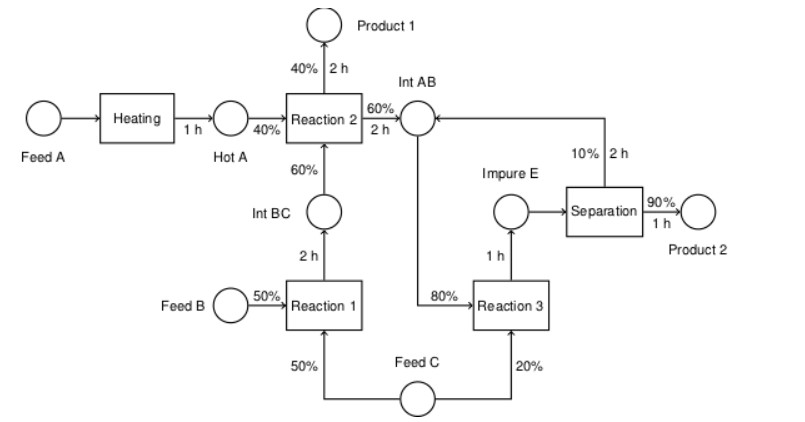
\includegraphics[width=1.0\textwidth]{пример процесса}
\label{fig:stn_exmp}
\end{figure}

Процессы (в особенности сетевые) удобно представлять себе в виде графов состояний (STN), впервые предложенных в работе \cite{stnoriginal}. Пример такого графа можно видеть на рисунке \ref{fig:stn_exmp}

\begin{figure}[h]
\caption{Классификация процессов}
\centering
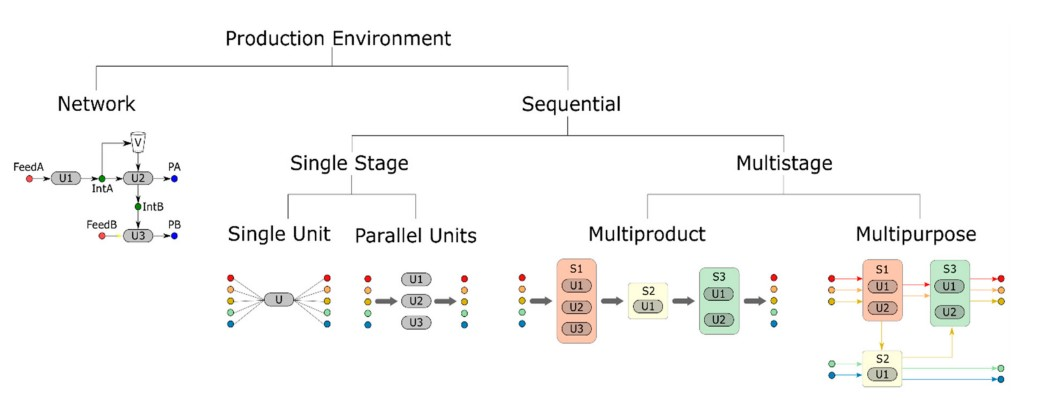
\includegraphics[width=1.0\textwidth]{классификация процессов}
\label{fig:clas_proc}
\end{figure}

Классификация \ref{fig:clas_proc} взята из \cite{reallife} где она является более подробной, но в этой статье параллелизм и наличие многих продуктов/прекурсоров являются параметрами модели. Основной вопрос состоит в том, как переход от последовательных процессов к сетевым изменяет модель и какие методы, изобретённые для последовательных моделей применимы к сетевым и наоборот. 

\section{Описание моделей}

Моделью в рамках данной работы будем называть задачу смешанного целочисленного линейного программирования в общей форме. На данном этапе необходимо закодировать решения, принимаемые системой составления расписаний в переменные, которые будут называться \textbf{решающими переменными}. Далее $T$ будет обозначать множество промежутков времени и переменные, с ним связанные. Другими большими латинскими буквами (с индексами) будут обозначаться непрерывные решающие переменные, малыми --- бинарные решающие переменные и индексы (в некоторых моделях бинарные переменные и являются своеобразными <<индексами>> того, что какое-то утверждение верно или нет). Также большими буквами будут обозначаться параметры модели и их множества. Строчные греческие буквы по умолчанию означают разные затраты, сопровождающие процесс (в моделях, где они присутствуют).

Опишем все обозначения, которые будут встречаться в эксперименте.

\begin{enumerate}
   \item Множества:
   \begin{itemize}
     \item $U$ --- множество производственных узлов. Индексы у этого множества означают:
     \begin{itemize}
     		\item $U_j$ --- узлы, способные производить задачу $j \in J$.
     \end{itemize}
     \item $P$ --- множество продуктов (как прекурсоры, так и те, что получаются в процессе реакций). Индексы у этого множества означают:
		\begin{itemize}
     		\item $P^{in}_j$ --- продукты, потребляемые задачей $j \in J$.
     		\item $P^{out}_j$ --- продукты, производимые задачей $j \in J$.
     		\item $P^{`}$ --- продукты, которые надо произвести к концу (заказ).
     \end{itemize}
     
     \item $T$ --- множество временных промежутков
     \item $J$ --- множество задач (задача есть производство некоторого вещества по его рецепту). Индексы у этого множества означают:
     \begin{itemize}
     		\item $J^{in}_p$ --- задачи, потребляющие продукт $p \in P$.
     		\item $J^{out}_p$ --- задачи, производящие продукт $p \in P$.
     		\item $J^{u}$ --- задачи, которые могут быть произведены на узле $u \in U$.
     \end{itemize}
   \end{itemize}
   \item Параметры:
   	\begin{itemize}
   		\item $B^{min}_u, B^{max}_u$ --- минимальный и максимальный размеры пакета для запуска узла $u \in U$.
   		\item $S^{max}_p$ --- максимальное количество продукта $p \in P$, которое может находиться на складе в любой момент времени.
   		\item $D_p$ --- внешние требования на производство продукта $p \in P^{`}$.
   		\item $I_p$ --- изначальное количество продукта $p \in P$ на складе.
   		\item $\Tau_{u, j}$ --- время работы задачи $j \in J$ на узле $u \in U$. По умолчанию считается, что время исполнения задачи не зависит от размера пакета. Будут рассмотренны случаи, в которых время может зависеть от размера пакета, в таком случае этот параметр значит <<время работы за килограмм входных веществ>>.
   		\item $\mathcal{Q}^{in}_{p, j}, \mathcal{Q}^{out}_{p, j}$ --- пропорции входного/выходного продукта $p \in P$ в пакете в рецепте задачи $j \in J$ в случае мультипотребления/мультипроизводства.
   		\item $\theta_{u}$ --- стоимость запуска оборудования $u \in U$ за единицу времени.
   		\item $\psi_{p}$ --- стоимость хранения продукта $p \in P$ на складе.
   		\item $\eta_{p, u}$ --- стоимость производства продукта $p \in P$ на узле $u \in U$ за килограмм.
   	\end{itemize}
\end{enumerate}

В моделях будут рассматриваться две целевые функции:
\begin{enumerate}
\item
\begin{equation}
\begin{gathered}
	min \: MS\\
	s.t.\\
	MS \leq T_{u, i} \: \forall u \in U, i \in \mathbb{N}
\end{gathered}
\end{equation}

Минимизация общего времени выполнения (makespan) при условиях, что оно больше, чем время окончания каждого запуска каждого узла. В зависимости от представления времени в модели величина справа будет по-разному выражаться из переменных.

\item 
\begin{equation}
\begin{gathered}
	min \: \displaystyle\sum_{p \in P, j \in J^{out}_p, u \in U_j, n \in \mathbb{N} }  \eta_{p, u} \mathcal{Q}^{out}_{p, j} B_{j, n} + \displaystyle\sum_{j \in J, u \in U_j, n \in \mathbb{N}} \Tau_{u, j}*\theta_{u}*x_{u, j, n} + \displaystyle\sum_{p \in P, t \in T} S_{p, j, t}\\
	s.t.\\
	S_{p, j, t} = \displaystyle\sum{j \in J^{out}_p, T{u, j} <= t}  B_{p, j, n} - \displaystyle\sum{j \in J^{in}_p, T{u, j} <= t}  B_{p, j, n}\\
	B^{min}_u \leq B_{p, j, n} \leq B^{max}_u \\
	 \forall p \in P, j \in J^{out}_p, u \in U_j, n \in \mathbb{N}
\end{gathered}
\end{equation}

Минимизация стоимости производства, в которую входит стоимость работы узлов за время, стоимость производства продуктов за массу и стоимость хранения продуктов. Параметры $B_{j, n}$ --- размер пакета, подаваемого на вход $n$-того запуска задачи $j$, $x_{u, j, n}$ --- индикатор того, что $n$-тый запуск задачи $j$ совершился на узле $u$ будут считаться в каждой модели по-своему (данные уравнения отражают суть целевых функций и будут отличаться в зависимости от подхода).


\item 
Минимизация некоторого общего показателя (например, взвешенной суммы), зависящего от стоимости издержек и временных затрат.

\end{enumerate}
\section{Модели}

\section{Заключение}
Желательно, чтобы этот раздел был, причём он не~должен дословно повторять аннотацию.
Обычно здесь отмечают, каких результатов удалось добиться, какие проблемы остались открытыми.

%%%% если имеется doi цитируемого источника, необходимо его указать, см. пример в \bibitem{article}
%%%% DOI публикации, зарегистрированной в системе Crossref, можно получить по адресу http://www.crossref.org/guestquery/
\begin{thebibliography}{99}

\bibitem{lpheuristic}
    \BibAuthor{F. Blomer, H.-O. Gunther}
    LP-based heuristics for scheduling chemical batch processes, 2010
    \BibJournal{International Journal of Production Research}, 38:5, 1029-1051
	\BibDoi{10.1080/002075400189004}.

\bibitem{dairy}
    \BibAuthor{Georgios P. Georgiadis, Georgios M. Kopanos, Antonis Karkaris, Harris Ksafopoulos and Michael C. Georgiadis}
    Optimal Production Scheduling in the Dairy Industries, 2019
    \BibJournal{Industrial \& Engineering Chemistry Research} 58 (16), 6537-6550
	\BibDoi{10.1021/acs.iecr.8b05710}.
	
\bibitem{reallife}
    \BibAuthor{Georgiadis, Georgios P. and Elekidis, Apostolos P. and Georgiadis, Michael C.}
    Optimization-Based Scheduling for the Process Industries: From Theory to Real-Life Industrial Applications, 2019
    \BibJournal{Industrial \& Engineering Chemistry Research} 58 (16), 6537-6550
	\BibDoi{10.3390/pr7070438}.
	
\bibitem{hybridizing}
    \BibAuthor{Siqun Wang, Monique Guignard}
    Hybridizing Discrete- and Continuous-Time Models For Batch Sizing and
Scheduling Problems, 2006
    \BibJournal{Computers \& Operations Research} Volume 33, Issue 4
	\BibDoi{10.1016/j.cor.2004.11.013}.
	
\bibitem{discretetime}
    \BibAuthor{Christos T. Maravelias and Ignacio E. Grossmann}
    Minimization of the Makespan with a Discrete-Time State-Task Network Formulation, 2003
    \BibJournal{Industrial \& Engineering Chemistry Research}
	\BibDoi{10.1021/ie034053b}.
	
\bibitem{stnoriginal}
    \BibAuthor{E.Kondili, C.C.Pantelides, R.W.H.Sargent}
    A general algorithm for short-term scheduling of batch operations—I. MILP formulation, 1993
    \BibJournal{Computers \& Chemical Engineering}
	\BibDoi{10.1021/ie034053b10.1016/0098-1354(93)80015-F}.
	
%\bibitem{webArticle}
%	\BibAuthor{Blaga~P.\,A.}
%	Commutative Diagrams with XY-pic II. Frames and Matrices~//
%	\BibJournal{PracTEX J.}, 2007. Vol.\,4.
%	URL: \BibUrl{https://tug.org/pracjourn/2007-1/blaga/blaga.pdf}.
%
%\bibitem{webResource}
%	XYpic.
%	URL: \BibUrl{http://akagi.ms.u-tokyo.ac.jp/input9.pdf}.
%	
%\bibitem{inproceedingsRus}
%	\BibAuthor{Усманов~Т.\,С., Гусманов~А.\,А., Муллагалин~И.\,З., Мухаметшина~Р.5\,Ю., Червякова~А.\,Н., Свешников~А.\,В.}
%	Особенности проектирования разработки месторождений с применением гидроразрыва пласта~//
%	\BibJournal{Труды 6-го Междунар. симп. <<Новые ресурсосберегающие технологии недропользования и повышения нефтегазоотдачи>>}.~---
%	М.:~Издательство, 2007. С.~267--272.

%\bibitem{inproceedingsEng}
 %   \BibAuthor{Author~N.}
  %  Paper title~//
   % \BibJournal{10th Conference (International) on Any Science Proceedings}.~---
    %Place of publication: Publisher, 2009. P.~111--122.

%\bibitem{techreport}
%	\BibAuthor{Lambert~P.}
 % 	\BibTitle{The title of the work}.
  %	Place of publication:~The institution that published, 1993.  Report~2.
 	
\end{thebibliography}

%%%% если имеется doi цитируемого источника, необходимо его указать, см. пример в \bibitem{article}
%%%% DOI публикации, зарегистрированной в системе Crossref, можно получить по адресу http://www.crossref.org/guestquery/.

\end{document}
